\documentclass[]{book}
\usepackage{lmodern}
\usepackage{amssymb,amsmath}
\usepackage{ifxetex,ifluatex}
\usepackage{fixltx2e} % provides \textsubscript
\ifnum 0\ifxetex 1\fi\ifluatex 1\fi=0 % if pdftex
  \usepackage[T1]{fontenc}
  \usepackage[utf8]{inputenc}
\else % if luatex or xelatex
  \ifxetex
    \usepackage{mathspec}
  \else
    \usepackage{fontspec}
  \fi
  \defaultfontfeatures{Ligatures=TeX,Scale=MatchLowercase}
\fi
% use upquote if available, for straight quotes in verbatim environments
\IfFileExists{upquote.sty}{\usepackage{upquote}}{}
% use microtype if available
\IfFileExists{microtype.sty}{%
\usepackage{microtype}
\UseMicrotypeSet[protrusion]{basicmath} % disable protrusion for tt fonts
}{}
\usepackage[margin=1in]{geometry}
\usepackage{hyperref}
\hypersetup{unicode=true,
            pdftitle={Metody przetwarzania i analizy danych w R},
            pdfauthor={Łukasz Wawrowski},
            pdfborder={0 0 0},
            breaklinks=true}
\urlstyle{same}  % don't use monospace font for urls
\usepackage{natbib}
\bibliographystyle{plainnat}
\usepackage{color}
\usepackage{fancyvrb}
\newcommand{\VerbBar}{|}
\newcommand{\VERB}{\Verb[commandchars=\\\{\}]}
\DefineVerbatimEnvironment{Highlighting}{Verbatim}{commandchars=\\\{\}}
% Add ',fontsize=\small' for more characters per line
\usepackage{framed}
\definecolor{shadecolor}{RGB}{248,248,248}
\newenvironment{Shaded}{\begin{snugshade}}{\end{snugshade}}
\newcommand{\KeywordTok}[1]{\textcolor[rgb]{0.13,0.29,0.53}{\textbf{#1}}}
\newcommand{\DataTypeTok}[1]{\textcolor[rgb]{0.13,0.29,0.53}{#1}}
\newcommand{\DecValTok}[1]{\textcolor[rgb]{0.00,0.00,0.81}{#1}}
\newcommand{\BaseNTok}[1]{\textcolor[rgb]{0.00,0.00,0.81}{#1}}
\newcommand{\FloatTok}[1]{\textcolor[rgb]{0.00,0.00,0.81}{#1}}
\newcommand{\ConstantTok}[1]{\textcolor[rgb]{0.00,0.00,0.00}{#1}}
\newcommand{\CharTok}[1]{\textcolor[rgb]{0.31,0.60,0.02}{#1}}
\newcommand{\SpecialCharTok}[1]{\textcolor[rgb]{0.00,0.00,0.00}{#1}}
\newcommand{\StringTok}[1]{\textcolor[rgb]{0.31,0.60,0.02}{#1}}
\newcommand{\VerbatimStringTok}[1]{\textcolor[rgb]{0.31,0.60,0.02}{#1}}
\newcommand{\SpecialStringTok}[1]{\textcolor[rgb]{0.31,0.60,0.02}{#1}}
\newcommand{\ImportTok}[1]{#1}
\newcommand{\CommentTok}[1]{\textcolor[rgb]{0.56,0.35,0.01}{\textit{#1}}}
\newcommand{\DocumentationTok}[1]{\textcolor[rgb]{0.56,0.35,0.01}{\textbf{\textit{#1}}}}
\newcommand{\AnnotationTok}[1]{\textcolor[rgb]{0.56,0.35,0.01}{\textbf{\textit{#1}}}}
\newcommand{\CommentVarTok}[1]{\textcolor[rgb]{0.56,0.35,0.01}{\textbf{\textit{#1}}}}
\newcommand{\OtherTok}[1]{\textcolor[rgb]{0.56,0.35,0.01}{#1}}
\newcommand{\FunctionTok}[1]{\textcolor[rgb]{0.00,0.00,0.00}{#1}}
\newcommand{\VariableTok}[1]{\textcolor[rgb]{0.00,0.00,0.00}{#1}}
\newcommand{\ControlFlowTok}[1]{\textcolor[rgb]{0.13,0.29,0.53}{\textbf{#1}}}
\newcommand{\OperatorTok}[1]{\textcolor[rgb]{0.81,0.36,0.00}{\textbf{#1}}}
\newcommand{\BuiltInTok}[1]{#1}
\newcommand{\ExtensionTok}[1]{#1}
\newcommand{\PreprocessorTok}[1]{\textcolor[rgb]{0.56,0.35,0.01}{\textit{#1}}}
\newcommand{\AttributeTok}[1]{\textcolor[rgb]{0.77,0.63,0.00}{#1}}
\newcommand{\RegionMarkerTok}[1]{#1}
\newcommand{\InformationTok}[1]{\textcolor[rgb]{0.56,0.35,0.01}{\textbf{\textit{#1}}}}
\newcommand{\WarningTok}[1]{\textcolor[rgb]{0.56,0.35,0.01}{\textbf{\textit{#1}}}}
\newcommand{\AlertTok}[1]{\textcolor[rgb]{0.94,0.16,0.16}{#1}}
\newcommand{\ErrorTok}[1]{\textcolor[rgb]{0.64,0.00,0.00}{\textbf{#1}}}
\newcommand{\NormalTok}[1]{#1}
\usepackage{longtable,booktabs}
\usepackage{graphicx,grffile}
\makeatletter
\def\maxwidth{\ifdim\Gin@nat@width>\linewidth\linewidth\else\Gin@nat@width\fi}
\def\maxheight{\ifdim\Gin@nat@height>\textheight\textheight\else\Gin@nat@height\fi}
\makeatother
% Scale images if necessary, so that they will not overflow the page
% margins by default, and it is still possible to overwrite the defaults
% using explicit options in \includegraphics[width, height, ...]{}
\setkeys{Gin}{width=\maxwidth,height=\maxheight,keepaspectratio}
\IfFileExists{parskip.sty}{%
\usepackage{parskip}
}{% else
\setlength{\parindent}{0pt}
\setlength{\parskip}{6pt plus 2pt minus 1pt}
}
\setlength{\emergencystretch}{3em}  % prevent overfull lines
\providecommand{\tightlist}{%
  \setlength{\itemsep}{0pt}\setlength{\parskip}{0pt}}
\setcounter{secnumdepth}{5}
% Redefines (sub)paragraphs to behave more like sections
\ifx\paragraph\undefined\else
\let\oldparagraph\paragraph
\renewcommand{\paragraph}[1]{\oldparagraph{#1}\mbox{}}
\fi
\ifx\subparagraph\undefined\else
\let\oldsubparagraph\subparagraph
\renewcommand{\subparagraph}[1]{\oldsubparagraph{#1}\mbox{}}
\fi

%%% Use protect on footnotes to avoid problems with footnotes in titles
\let\rmarkdownfootnote\footnote%
\def\footnote{\protect\rmarkdownfootnote}

%%% Change title format to be more compact
\usepackage{titling}

% Create subtitle command for use in maketitle
\newcommand{\subtitle}[1]{
  \posttitle{
    \begin{center}\large#1\end{center}
    }
}

\setlength{\droptitle}{-2em}

  \title{Metody przetwarzania i analizy danych w R}
    \pretitle{\vspace{\droptitle}\centering\huge}
  \posttitle{\par}
    \author{Łukasz Wawrowski}
    \preauthor{\centering\large\emph}
  \postauthor{\par}
    \date{}
    \predate{}\postdate{}
  
\usepackage{booktabs}
\usepackage{amsthm}
\makeatletter
\def\thm@space@setup{%
  \thm@preskip=8pt plus 2pt minus 4pt
  \thm@postskip=\thm@preskip
}
\makeatother

\begin{document}
\maketitle

{
\setcounter{tocdepth}{1}
\tableofcontents
}
\chapter*{Wprowadzenie}\label{wprowadzenie}
\addcontentsline{toc}{chapter}{Wprowadzenie}

Literatura podstawowa:

\begin{itemize}
\tightlist
\item
  Przemysław Biecek -
  \href{http://pbiecek.github.io/Przewodnik/}{\emph{Przewodnik po
  pakiecie R}}
\item
  Marek Gągolewski -
  \href{http://www.gagolewski.com/publications/programowanier/}{\emph{Programowanie
  w języku R. Analiza danych, obliczenia, symulacje.}}
\item
  Garret Grolemund, Hadley Wickham -
  \href{http://r4ds.had.co.nz/}{\emph{R for Data Science}}
  (\href{https://helion.pl/ksiazki/jezyk-r-kompletny-zestaw-narzedzi-dla-analitykow-danych-hadley-wickham-garrett-grolemund,jezrko.htm}{polska
  wersja})
\end{itemize}

Literatura dodatkowa:

\begin{itemize}
\tightlist
\item
  \href{https://github.com/mi2-warsaw/SER/blob/master/histoRia/README.md}{inne
  pozycje po polsku}
\item
  \href{https://bookdown.org/}{inne pozycje po angielsku}
\end{itemize}

Internet:

\begin{itemize}
\tightlist
\item
  \href{https://www.r-bloggers.com/}{R-bloggers}
\item
  \href{https://rweekly.org/}{rweekly}
\end{itemize}

\chapter{Wprowadzenie}\label{wprowadzenie-1}

\section{Narzędzie}\label{narzedzie}

\begin{itemize}
\tightlist
\item
  darmowe
\item
  wszechstronne
\item
  wsparcie społeczności
\item
  wersja desktopowa i serwerowa
\end{itemize}

czyli \textbf{R} - środowisko do obliczeń statystycznych i wizualizacji
wyników

\begin{itemize}
\tightlist
\item
  strona projektu: \href{https://www.r-project.org/}{r-project.org}
\item
  świetne IDE: \href{https://www.rstudio.com/}{RStudio}
\item
  wersja przeglądarkowa: \href{https://rstudio.cloud/}{rstudio.cloud}
\end{itemize}

\href{https://www.business-science.io/business/2018/10/08/python-and-r.html}{R
+ Python}

\section{Cele analiz}\label{cele-analiz}

Podstawowe:

\begin{itemize}
\tightlist
\item
  wnioskowanie statystyczne - porównywanie grup
\item
  regresja - poszukiwanie związków
\item
  klasyfikacja - przyporządkowanie do grup
\item
  grupowanie - poszukiwanie grup
\item
  prognozowanie - patrzenie w przyszłość
\end{itemize}

Inne:

\begin{itemize}
\tightlist
\item
  analiza języka naturalnego
\item
  rozpoznawanie obrazów
\item
  analiza koszykowa
\item
  \ldots{}
\end{itemize}

\subsection{Eksporacja danych}\label{eksporacja-danych}

Pakiet \texttt{tidyverse}

\begin{Shaded}
\begin{Highlighting}[]
\KeywordTok{library}\NormalTok{(tidyverse)}
\end{Highlighting}
\end{Shaded}

\begin{itemize}
\tightlist
\item
  analiza częstości dla zmiennych jakościowych
\item
  analiza struktury dla zmiennych ilościowych
\end{itemize}

Case study: \href{data/wybory2018.xlsx}{Wybory 2018}

\chapter{Testowanie hipotez}\label{testowanie-hipotez}

\section{Hipoteza statystyczna}\label{hipoteza-statystyczna}

Przypuszczenie dotyczące własności analizowanej cechy, np. średnia w
populacji jest równa 10, rozkład cechy jest normalny.

Formułuje się zawsze dwie hipotezy: hipotezę zerową (\(H_0\)) i hipotezę
alternatywną (\(H_1\)). Hipoteza zerowa jest hipotezą mówiącą o
równości:

\(H_0: \bar{x}=10\)

Z kolei hipoteza alternatywna zakłada coś przeciwnego:

\(H_1: \bar{x}\neq 10\)

Zamiast znaku nierówności (\(\neq\)) może się także pojawić znak
mniejszości (\(<\)) lub większości (\(>\)).

\section{Poziom istotności i wartość
p}\label{poziom-istotnosci-i-wartosc-p}

Hipotezy statystyczne weryfikuje się przy określonym poziomie istotności
\(\alpha\), który wskazuje maksymalny poziom akceptowalnego błędu
(najczęściej \(\alpha=0,05\)).

Większość programów statystycznych podaje w wynikach testu wartość
p.~Jest to prawdopodobieństwo uzyskania obserwowanych wyników przy
założeniu prawdziwości hipotezy zerowej.

Generalnie jeśli \(p < \alpha\) - odrzucamy hipotezę zerową.

\href{http://idane.pl/blog/asa}{Krytyka wartości p}

\section{Testy parametryczne i
nieparametryczne}\label{testy-parametryczne-i-nieparametryczne}

Testy statystyczne dzielą się na dwie grupy:

\begin{itemize}
\tightlist
\item
  parametryczne, które wymagają spełnienia założeń, ale są
  dokładniejsze,
\item
  nieparametryczne, które nie wymagają tylu założeń, ale są mniej
  dokładne.
\end{itemize}

\chapter{Regresja}\label{regresja}

\section{Regresja prosta}\label{regresja-prosta}

Na podstawie \href{data/Salary_Data.csv}{danych} dotyczących informacji
o doświadczeniu i wynagrodzeniu pracowników zbuduj model określający
`widełki' dla potencjalnych pracowników o doświadczeniu równym 8, 10 i
11 lat.

\href{res/regresja_prosta.Rmd}{regresja\_prosta.Rmd}

\href{res/adr.zip}{cały projekt}

\subsection{Zadanie}\label{zadanie}

Dla danych dotyczących \href{data/sklep77.csv}{sklepu nr 77} opracuj
model zależności sprzedaży od liczby klientów. Ile wynosi teoretyczna
sprzedaż w dniach, w których liczba klientów będzie wynosiła 560, 740,
811 oraz 999 osób?

\section{Regresja wieloraka}\label{regresja-wieloraka}

Na podstawie danych dotyczących
\href{data/pracownicy.xlsx}{zatrudnienia} opracuj model, w którym
zmienną zależną jest bieżące wynagrodzenie. Jaka cecha ma największy
wpływ na tę wartość?

Opis zbioru:

\begin{itemize}
\tightlist
\item
  id - kod pracownika
\item
  plec - płeć pracownika (0 - mężczyzna, 1 - kobieta)
\item
  data\_urodz - data urodzenia
\item
  edukacja - wykształcenie (w latach nauki)
\item
  kat\_pracownika - grupa pracownicza (1 - ochroniarz, 2 - urzędnik, 3 -
  menedżer)
\item
  bwynagrodzenie - bieżące wynagrodzenie
\item
  pwynagrodzenie - początkowe wynagrodzenie
\item
  staz - staż pracy (w miesiącach)
\item
  doswiadczenie - poprzednie zatrudnienie (w miesiącach)
\item
  zwiazki - przynależność do związków zawodowych (0 - nie, 1 - tak)
\item
  wiek - wiek (w latach)
\end{itemize}

Wczytanie bibliotek \texttt{tidyverse}, \texttt{readxl} oraz danych.

\begin{Shaded}
\begin{Highlighting}[]
\KeywordTok{library}\NormalTok{(tidyverse)}
\KeywordTok{library}\NormalTok{(readxl)}

\KeywordTok{options}\NormalTok{(}\DataTypeTok{scipen =} \DecValTok{100}\NormalTok{)}

\NormalTok{pracownicy <-}\StringTok{ }\KeywordTok{read_xlsx}\NormalTok{(}\StringTok{"data/pracownicy.xlsx"}\NormalTok{)}

\NormalTok{pracownicy2 <-}\StringTok{ }\NormalTok{pracownicy }\OperatorTok
\StringTok{  }\KeywordTok{filter}\NormalTok{(}\OperatorTok{!}\KeywordTok{is.na}\NormalTok{(wiek)) }\OperatorTok
\StringTok{  }\KeywordTok{select}\NormalTok{(}\OperatorTok{-}\NormalTok{id, }\OperatorTok{-}\NormalTok{data_urodz) }\OperatorTok
\StringTok{  }\KeywordTok{mutate}\NormalTok{(}\DataTypeTok{plec=}\KeywordTok{as.factor}\NormalTok{(plec),}
         \DataTypeTok{kat_pracownika=}\KeywordTok{as.factor}\NormalTok{(kat_pracownika),}
         \DataTypeTok{zwiazki=}\KeywordTok{as.factor}\NormalTok{(zwiazki))}

\KeywordTok{summary}\NormalTok{(pracownicy2)}
\end{Highlighting}
\end{Shaded}

\begin{verbatim}
##  plec       edukacja     kat_pracownika bwynagrodzenie   pwynagrodzenie 
##  0:257   Min.   : 8.00   1:362          Min.   : 15750   Min.   : 9000  
##  1:216   1st Qu.:12.00   2: 27          1st Qu.: 24000   1st Qu.:12450  
##          Median :12.00   3: 84          Median : 28800   Median :15000  
##          Mean   :13.49                  Mean   : 34418   Mean   :17009  
##          3rd Qu.:15.00                  3rd Qu.: 37050   3rd Qu.:17490  
##          Max.   :21.00                  Max.   :135000   Max.   :79980  
##       staz       doswiadczenie    zwiazki      wiek      
##  Min.   :63.00   Min.   :  0.00   0:369   Min.   :24.00  
##  1st Qu.:72.00   1st Qu.: 19.00   1:104   1st Qu.:30.00  
##  Median :81.00   Median : 55.00           Median :33.00  
##  Mean   :81.14   Mean   : 95.95           Mean   :38.67  
##  3rd Qu.:90.00   3rd Qu.:139.00           3rd Qu.:47.00  
##  Max.   :98.00   Max.   :476.00           Max.   :66.00
\end{verbatim}

W zmiennej wiek występował brak danych, który został usunięty. Usunięto
także kolumny, które nie przydadzą się w modelowaniu. Ponadto dokonujemy
przekształcenia typu cech, które są jakościowe (płeć, kat\_pracownika,
zwiazki) z typu liczbowego na czynnik/faktor, który będzie poprawnie
interpretowany przez model.

W modelu zmienna zależna to \texttt{bwynagrodzenie}, natomiast jako
zmienne niezależne bierzemy pod uwagę wszystkie pozostałe cechy.

\begin{Shaded}
\begin{Highlighting}[]
\NormalTok{model <-}\StringTok{ }\KeywordTok{lm}\NormalTok{(bwynagrodzenie }\OperatorTok{~}\StringTok{ }\NormalTok{., pracownicy2)}
\KeywordTok{summary}\NormalTok{(model)}
\end{Highlighting}
\end{Shaded}

\begin{verbatim}
## 
## Call:
## lm(formula = bwynagrodzenie ~ ., data = pracownicy2)
## 
## Residuals:
##    Min     1Q Median     3Q    Max 
## -23185  -3041   -705   2591  46295 
## 
## Coefficients:
##                    Estimate  Std. Error t value             Pr(>|t|)    
## (Intercept)     -4764.87418  3590.49652  -1.327              0.18514    
## plec1           -1702.43743   796.51779  -2.137              0.03309 *  
## edukacja          482.43603   160.83977   2.999              0.00285 ** 
## kat_pracownika2  6643.17910  1638.06138   4.056  0.00005869172850407 ***
## kat_pracownika3 11169.64519  1372.73990   8.137  0.00000000000000377 ***
## pwynagrodzenie      1.34021     0.07317  18.315 < 0.0000000000000002 ***
## staz              154.50876    31.65933   4.880  0.00000145958620443 ***
## doswiadczenie     -15.77375     5.78369  -2.727              0.00663 ** 
## zwiazki1        -1011.55276   787.80884  -1.284              0.19978    
## wiek              -64.78787    47.88015  -1.353              0.17668    
## ---
## Signif. codes:  0 '***' 0.001 '**' 0.01 '*' 0.05 '.' 0.1 ' ' 1
## 
## Residual standard error: 6809 on 463 degrees of freedom
## Multiple R-squared:  0.8444, Adjusted R-squared:  0.8414 
## F-statistic: 279.1 on 9 and 463 DF,  p-value: < 0.00000000000000022
\end{verbatim}

Tak zbudowany model wyjaśnia 84\% zmienności bieżącego wynagrodzenia,
ale nie wszystkie zmienne są w tym modelu istotne.

Parametry regresji mają następujące interpretacje:

\begin{itemize}
\tightlist
\item
  plec1 - kobiety zarabiają przeciętnie o 1702,44 zł mniej niż
  mężczyźni,
\item
  edukacja - wzrost liczby lat nauki o rok powoduje średni wzrost
  bieżącego wynagrodzenia o 482,44 zł
\item
  kat\_pracownika2 - pracownicy o kodzie 2 (urzędnik) zarabiają średnio
  o 6643,18 zł więcej niż pracownik o kodzie 1 (ochroniarz)
\item
  kat\_pracownika2 - pracownicy o kodzie 3 (menedżer) zarabiają średnio
  o 11169,65 zł więcej niż pracownik o kodzie 1 (ochroniarz)
\item
  pwynagrodzenie - wzrost początkowego wynagrodzenia o 1 zł powoduje
  przecięny wzrost bieżącego wynagrodzenia o 1,34 zł
\item
  staz - wzrost stażu pracy o miesiąc skutkuje przeciętnym wzrostem
  bieżącego wynagrodzenia o 154,51 zł
\item
  doswiadcznie - wzrost doświadczenia o miesiąc powoduje średni spadek
  bieżącego wynagrodzenia o 15,77 zł
\item
  zwiazki1 - pracownicy należący do związków zawodowych zarabiają
  średnio o 1011,55 zł mniej aniżeli pracownicy, którzy do związków nie
  zależą
\item
  wiek - wzrost wieku pracownika o 1 rok to przecięnym spadek bieżącego
  wynagrodzenia o 64,79 zł
\end{itemize}

Wszystkie te zależności obowiązują przy założeniu \emph{ceteris paribus}
- przy pozostałych warunkach niezmienionych.

Ten model wymaga oczywiście ulepszenie do czego wykorzystamy m.in.
pakiet
\href{https://cran.r-project.org/web/packages/olsrr/index.html}{olsrr}.

Pierwszą kwestią, którą się zajmiemy jest współliniowość zmiennych. W
regresji zmienne objaśniające powinny być jak najbardziej skorelowane ze
zmienną objaśnianą, a możliwie nieskorelowane ze sobą. W związku z tym
wybieramy ze zbioru wyłącznie cechy ilościowe, dla którym wyznaczymy
współczynnik korelacji liniowej Pearsona.

\begin{Shaded}
\begin{Highlighting}[]
\KeywordTok{library}\NormalTok{(corrplot)}
\KeywordTok{library}\NormalTok{(olsrr)}

\NormalTok{korelacje <-}\StringTok{ }\NormalTok{pracownicy2 }\OperatorTok
\StringTok{  }\KeywordTok{select}\NormalTok{(}\OperatorTok{-}\KeywordTok{c}\NormalTok{(plec, kat_pracownika, zwiazki)) }\OperatorTok
\StringTok{  }\KeywordTok{cor}\NormalTok{()}

\KeywordTok{corrplot}\NormalTok{(korelacje, }\DataTypeTok{method =} \StringTok{"number"}\NormalTok{, }\DataTypeTok{type =} \StringTok{"upper"}\NormalTok{)}
\end{Highlighting}
\end{Shaded}

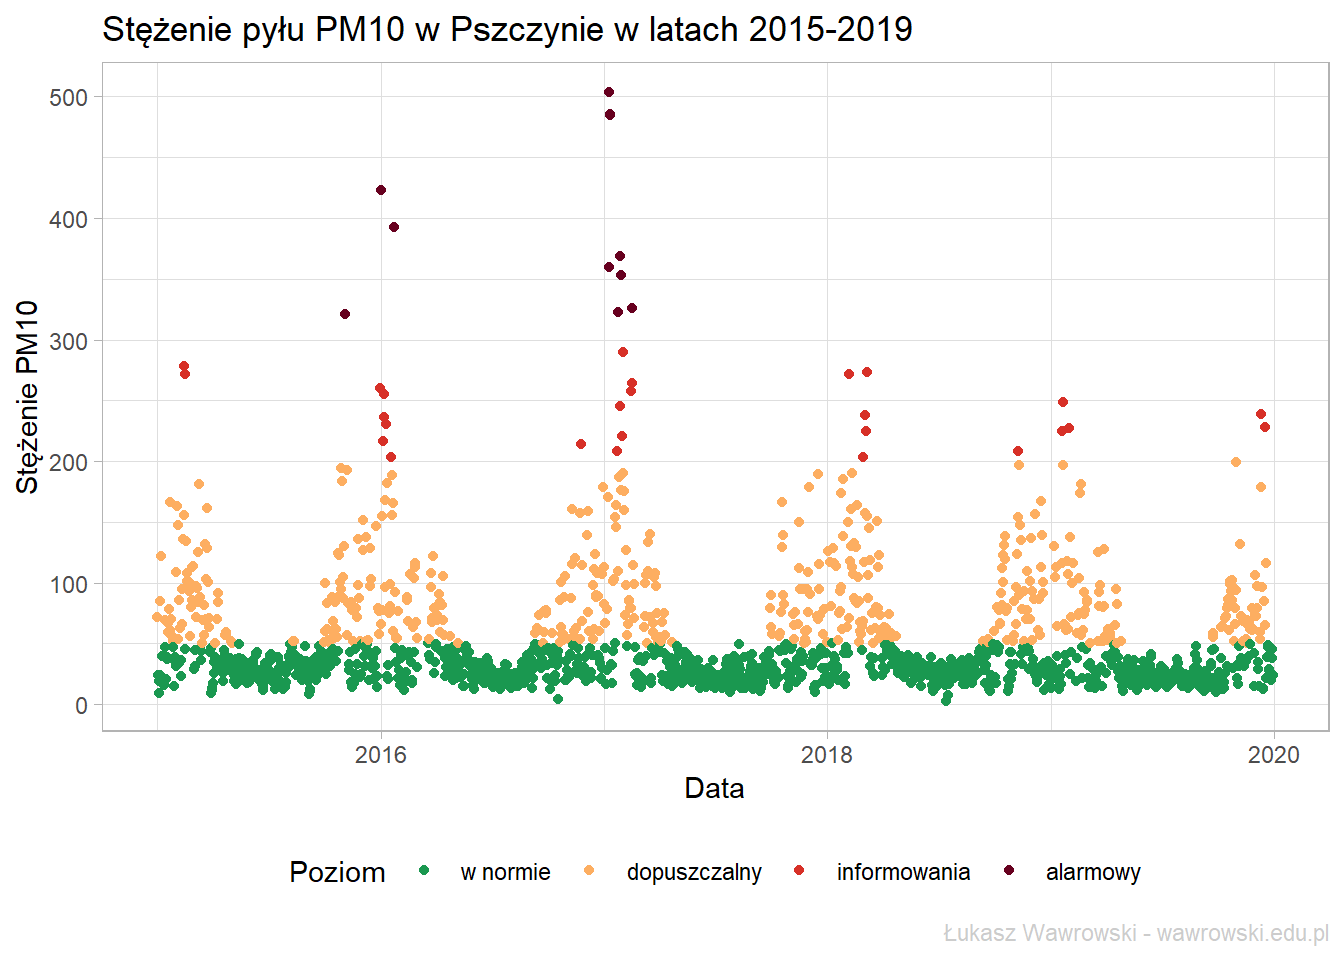
\includegraphics{Wawrowski_ADR_files/figure-latex/unnamed-chunk-4-1.pdf}

Możemy zauważyć, że wartości bieżącego wynagrodzenia są najsilniej
skorelowane w wartościami wynagrodzenia początkowego. Także
doświadczenie i wiek są silnie ze sobą związane, co może sugerować, że
obie zmienne wnoszą do modelu podobną informację.

W związku z tym powinniśmy wyeliminować niektóre zmienne z modelu
pozostawiając te najważniejsze. Wyróżnia się trzy podjeścia do tego
zagadnienia:

\begin{itemize}
\tightlist
\item
  ekspercki dobór cech,
\item
  budowa wszystkich możliwych modeli i wybór najlepszego według
  określonego kryterium,
\item
  regresja krokowa.
\end{itemize}

W przypadku budowy wszystkich możliwych modeli należy pamiętać o
rosnącej wykładniczo liczbie modeli - \(2^p-1\), gdzie \(p\) oznacza
liczbę zmiennych objaśniających. w rozważanym przypadku liczba modeli
wynosi 255.

\begin{Shaded}
\begin{Highlighting}[]
\NormalTok{wszystkie_modele <-}\StringTok{ }\KeywordTok{ols_step_all_possible}\NormalTok{(model)}
\end{Highlighting}
\end{Shaded}

W uzyskanym zbiorze danych są informacje o numerze modelu, liczbie
użytych zmiennych, nazwie tych zmiennych oraz wiele miar jakości. Te,
które warto wziąć pod uwagę to przede wszystkim:

\begin{itemize}
\tightlist
\item
  \texttt{rsquare} - współczynnik R-kwadrat,
\item
  \texttt{aic} - kryterium informacyjne Akaike,
\item
  \texttt{msep} - błąd średniokwadratowy predykcji.
\end{itemize}

Najwyższa wartość współczynnika \(R^2\) związana jest z modelem
zawierającym wszystkie dostępne zmienne objaśniające. Jest to pewna
niedoskonałość tej miary, która rośnie wraz z liczbą zmiennych w modelu,
nawet jeśli te zmienne nie są istotne.

W przypadku kryteriów informacyjnych oraz błędu średniokwadratowego
interesują nas jak najmniejsze wartości. Wówczas jako najlepszy należy
wskazać model nr 219 zawierający 6 zmiennych objaśniających.

Metodą, która także pozwoli uzyskać optymalny model, ale przy mniejszym
obciążeniu obliczeniowym jest regresja krokowa polegająca na krokowym
budowaniu modelu.

\begin{Shaded}
\begin{Highlighting}[]
\KeywordTok{ols_step_both_aic}\NormalTok{(model)}
\end{Highlighting}
\end{Shaded}

\begin{verbatim}
## Stepwise Selection Method 
## -------------------------
## 
## Candidate Terms: 
## 
## 1 . plec 
## 2 . edukacja 
## 3 . kat_pracownika 
## 4 . pwynagrodzenie 
## 5 . staz 
## 6 . doswiadczenie 
## 7 . zwiazki 
## 8 . wiek 
## 
## 
## Variables Entered/Removed: 
## 
## - pwynagrodzenie added 
## - kat_pracownika added 
## - doswiadczenie added 
## - staz added 
## - edukacja added 
## - plec added 
## 
## No more variables to be added or removed.
\end{verbatim}

\begin{verbatim}
## 
## 
##                                            Stepwise Summary                                            
## -----------------------------------------------------------------------------------------------------
## Variable           Method       AIC             RSS               Sum Sq          R-Sq      Adj. R-Sq 
## -----------------------------------------------------------------------------------------------------
## pwynagrodzenie    addition    9862.260    31053506813.535    106862706669.340    0.77484      0.77436 
## kat_pracownika    addition    9786.152    26215474648.689    111700738834.186    0.80992      0.80870 
## doswiadczenie     addition    9743.487    23853248017.651    114062965465.224    0.82705      0.82557 
## staz              addition    9719.469    22576592070.620    115339621412.255    0.83630      0.83455 
## edukacja          addition    9707.338    21912088629.084    116004124853.791    0.84112      0.83907 
## plec              addition    9703.188    21629051655.016    116287161827.859    0.84317      0.84081 
## -----------------------------------------------------------------------------------------------------
\end{verbatim}

Otrzymany w ten sposób model jest tożsamy z modelem charakteryzującym
się najlepszymi miarami jakości spośród zbioru wszystkich możliwych
modeli:

\begin{Shaded}
\begin{Highlighting}[]
\NormalTok{wybrany_model <-}\StringTok{ }\KeywordTok{lm}\NormalTok{(bwynagrodzenie }\OperatorTok{~}\StringTok{ }\NormalTok{pwynagrodzenie }\OperatorTok{+}\StringTok{ }\NormalTok{kat_pracownika }\OperatorTok{+}\StringTok{ }\NormalTok{doswiadczenie }\OperatorTok{+}\StringTok{ }\NormalTok{staz }\OperatorTok{+}\StringTok{ }\NormalTok{plec }\OperatorTok{+}\StringTok{ }\NormalTok{edukacja, }\DataTypeTok{data =}\NormalTok{ pracownicy2)}
\KeywordTok{summary}\NormalTok{(wybrany_model)}
\end{Highlighting}
\end{Shaded}

\begin{verbatim}
## 
## Call:
## lm(formula = bwynagrodzenie ~ pwynagrodzenie + kat_pracownika + 
##     doswiadczenie + staz + plec + edukacja, data = pracownicy2)
## 
## Residuals:
##    Min     1Q Median     3Q    Max 
## -22922  -3300   -673   2537  46524 
## 
## Coefficients:
##                  Estimate Std. Error t value             Pr(>|t|)    
## (Intercept)     -6547.147   3402.860  -1.924              0.05496 .  
## pwynagrodzenie      1.342      0.073  18.382 < 0.0000000000000002 ***
## kat_pracownika2  6734.992   1631.122   4.129   0.0000431843301918 ***
## kat_pracownika3 11226.635   1368.413   8.204   0.0000000000000023 ***
## doswiadczenie     -22.302      3.571  -6.246   0.0000000009514655 ***
## staz              147.865     31.461   4.700   0.0000034337703087 ***
## plec1           -1878.949    761.703  -2.467              0.01399 *  
## edukacja          501.391    160.270   3.128              0.00187 ** 
## ---
## Signif. codes:  0 '***' 0.001 '**' 0.01 '*' 0.05 '.' 0.1 ' ' 1
## 
## Residual standard error: 6820 on 465 degrees of freedom
## Multiple R-squared:  0.8432, Adjusted R-squared:  0.8408 
## F-statistic: 357.1 on 7 and 465 DF,  p-value: < 0.00000000000000022
\end{verbatim}

Uzyskany model charakteryzuje się mniejszym błędem standardowym od
modelu ze wszystkimi zmiennymi i tylko jedną nieistotną zmienną. Wyraz
wolny (Intercept) nie musi być istotny w modelu.

Wróćmy jeszcze na chwilę do tematu współliniowości zmiennych
objaśniających:

\begin{Shaded}
\begin{Highlighting}[]
\KeywordTok{ols_vif_tol}\NormalTok{(wybrany_model)}
\end{Highlighting}
\end{Shaded}

\begin{verbatim}
## # A tibble: 7 x 3
##   Variables       Tolerance   VIF
##   <chr>               <dbl> <dbl>
## 1 pwynagrodzenie      0.298  3.36
## 2 kat_pracownika2     0.687  1.46
## 3 kat_pracownika3     0.360  2.78
## 4 doswiadczenie       0.705  1.42
## 5 staz                0.986  1.01
## 6 plec1               0.683  1.46
## 7 edukacja            0.461  2.17
\end{verbatim}

Współczynnik tolerancji wskazuje na procent niewyjaśnionej zmienności
danej zmiennej przez pozostałe zmienne objaśniające. Przykładowo
współcznnik tolerancji dla początkowego wynagrodzenia wynosi 0,3371, co
oznacza, że 33\% zmienności początkowego wynagrodzenia nie jest
wyjaśnione przez pozostałe zmienne w modelu. Z kolei współczynnik VIF
jest obliczany na podstawie wartości współczynnika tolerancji i wskazuje
o ile wariancja szacowanego współcznnika regresji jest podwyższona z
powodu współliniowości danej zmiennej objaśniającej z pozostałymi
zmiennymi objaśniającymi. Wartość współczynnika VIF powyżej 4 należy
uznać za wskazującą na współliniowość. W analizowanym przypadku takie
zmienne nie występują.

Ocena siły wpływu poszczególnych zmiennych objaśniających na zmienną
objaśnianą w oryginalnej postaci modelu nie jest możliwa. Należy
wyznaczyć standaryzowane współczynniki beta, które wyliczane są na
danych standaryzowanych, czyli takich, które są pozbawione jednostek i
cechują się średnią równą 0, a odchyleniem standardowym równym 1.
Standaryzacja ma sens tylko dla cech numerycznych, w związku z czym
korzystamy z funkcji \texttt{mutate\_if()}, która jako pierwszy argument
przyjmuje warunek, który ma być spełniony, aby była zastosowane
przekształcenie podawane jako drugi argument.

\begin{Shaded}
\begin{Highlighting}[]
\NormalTok{pracownicy2_std <-}\StringTok{ }\NormalTok{pracownicy2 }\OperatorTok
\StringTok{  }\KeywordTok{mutate_if}\NormalTok{(is.numeric, }\KeywordTok{funs}\NormalTok{(scale))}

\NormalTok{wybrany_model_std <-}\StringTok{ }\KeywordTok{lm}\NormalTok{(bwynagrodzenie }\OperatorTok{~}\StringTok{ }\NormalTok{pwynagrodzenie }\OperatorTok{+}\StringTok{ }\NormalTok{kat_pracownika }\OperatorTok{+}\StringTok{ }
\StringTok{                          }\NormalTok{doswiadczenie }\OperatorTok{+}\StringTok{ }\NormalTok{staz }\OperatorTok{+}\StringTok{ }\NormalTok{plec }\OperatorTok{+}\StringTok{ }\NormalTok{edukacja, }\DataTypeTok{data =}\NormalTok{ pracownicy2_std)}
\KeywordTok{summary}\NormalTok{(wybrany_model_std)}
\end{Highlighting}
\end{Shaded}

\begin{verbatim}
## 
## Call:
## lm(formula = bwynagrodzenie ~ pwynagrodzenie + kat_pracownika + 
##     doswiadczenie + staz + plec + edukacja, data = pracownicy2_std)
## 
## Residuals:
##      Min       1Q   Median       3Q      Max 
## -1.34098 -0.19306 -0.03939  0.14841  2.72171 
## 
## Coefficients:
##                 Estimate Std. Error t value             Pr(>|t|)    
## (Intercept)     -0.08893    0.03144  -2.828              0.00488 ** 
## pwynagrodzenie   0.61842    0.03364  18.382 < 0.0000000000000002 ***
## kat_pracownika2  0.39400    0.09542   4.129   0.0000431843301918 ***
## kat_pracownika3  0.65677    0.08005   8.204   0.0000000000000023 ***
## doswiadczenie   -0.13657    0.02187  -6.246   0.0000000009514655 ***
## staz             0.08691    0.01849   4.700   0.0000034337703087 ***
## plec1           -0.10992    0.04456  -2.467              0.01399 *  
## edukacja         0.08464    0.02706   3.128              0.00187 ** 
## ---
## Signif. codes:  0 '***' 0.001 '**' 0.01 '*' 0.05 '.' 0.1 ' ' 1
## 
## Residual standard error: 0.399 on 465 degrees of freedom
## Multiple R-squared:  0.8432, Adjusted R-squared:  0.8408 
## F-statistic: 357.1 on 7 and 465 DF,  p-value: < 0.00000000000000022
\end{verbatim}

Spośród cech ilościowych największy wpływ na zmienną objaśnianą mają
wartości wynagrodzenia początkowego, staż, edukacja i na końcu
doświadczenie.

Reszty czyli różnice pomiędzy obserwowanymi wartościami zmiennej
objaśnianej, a wartościami wynikającymi z modelu w klasycznej metodzie
najmniejszych kwadratów powinny być zbliżone do rozkładu normalnego.
Oznacza to, że najwięcej reszt powinno skupiać się wokół zerowych
różnic, natomiast jak najmniej powinno być wartości modelowych znacznie
różniących się od tych rzeczywistych.

\begin{Shaded}
\begin{Highlighting}[]
\KeywordTok{ols_plot_resid_hist}\NormalTok{(wybrany_model)}
\end{Highlighting}
\end{Shaded}

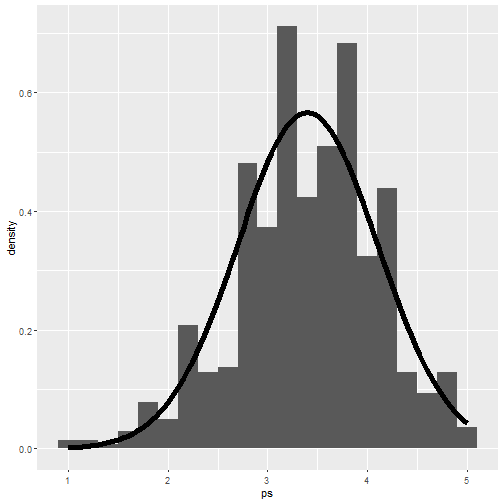
\includegraphics{Wawrowski_ADR_files/figure-latex/unnamed-chunk-10-1.pdf}

Reszty w naszym modelu wydają się być zbliżone do rozkładu normalnego.
Jednoznaczą odpowiedź da jednak odpowiedni test.

\begin{Shaded}
\begin{Highlighting}[]
\KeywordTok{ols_test_normality}\NormalTok{(wybrany_model)}
\end{Highlighting}
\end{Shaded}

\begin{verbatim}
## -----------------------------------------------
##        Test             Statistic       pvalue  
## -----------------------------------------------
## Shapiro-Wilk              0.868          0.0000 
## Kolmogorov-Smirnov        0.1092         0.0000 
## Cramer-von Mises         42.5504         0.0001 
## Anderson-Darling         13.0233         0.0000 
## -----------------------------------------------
\end{verbatim}

Hipoteza zerowa w tych testach mówi o zgodności rozkładu reszt z
rozkładem normalnym. Na podstawie wartości p, które są mniejsze od
\(\alpha=0,05\) stwierdzamy, że są podstawy do odrzucenia tej hipotezy
czyli reszty z naszego modelu nie mają rozkładu normalnego. W
diagnostyce przyczyn takiego stanu rzeczy pomoże nam wykres
kwantyl-kwantyl:

\begin{Shaded}
\begin{Highlighting}[]
\KeywordTok{ols_plot_resid_qq}\NormalTok{(wybrany_model)}
\end{Highlighting}
\end{Shaded}

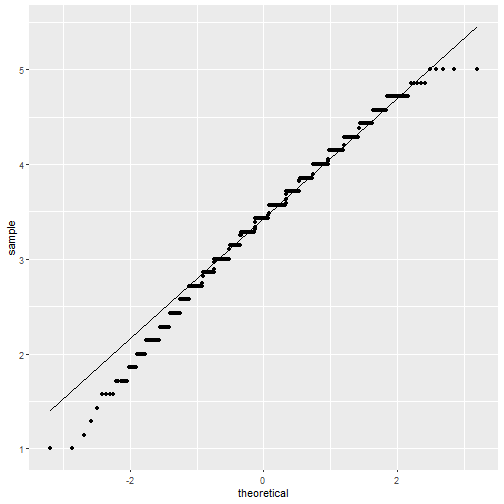
\includegraphics{Wawrowski_ADR_files/figure-latex/unnamed-chunk-12-1.pdf}

Gdyby wszystkie punkty leżały na prostej to oznaczałoby to normalność
rozkładu reszt. Tymczasem po lewej i prawej stronie tego wykresu
znajdują się potencjalne wartości odstające, które znacznie wpływają na
rozkład reszt modelu.

Wartości odstające można ustalić na podstawie wielu kryteriów. Do
jednych z najbardziej popularnych należy odległość Cooka:

\begin{Shaded}
\begin{Highlighting}[]
\NormalTok{cook <-}\StringTok{ }\KeywordTok{ols_plot_cooksd_bar}\NormalTok{(wybrany_model)}
\end{Highlighting}
\end{Shaded}

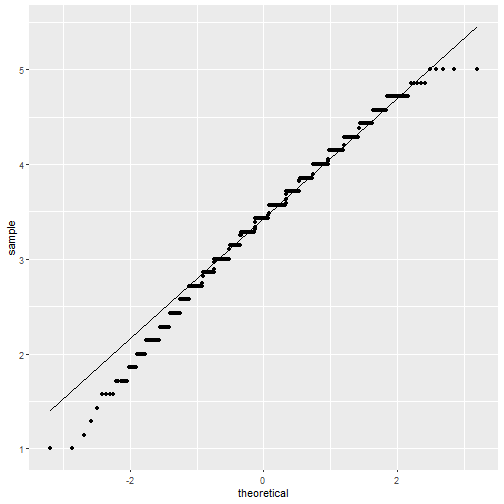
\includegraphics{Wawrowski_ADR_files/figure-latex/unnamed-chunk-13-1.pdf}

Przypisanie tej funkcji do obiektu zwraca nam tabelę z numerami
zidentyfikowanych obserwacji wpływowych. W przypadku odległości Cooka
jest to 12 obserwacji.

Inną miarą są reszty studentyzowane.

\begin{Shaded}
\begin{Highlighting}[]
\NormalTok{stud3 <-}\StringTok{ }\KeywordTok{ols_plot_resid_stud}\NormalTok{(wybrany_model)}
\end{Highlighting}
\end{Shaded}

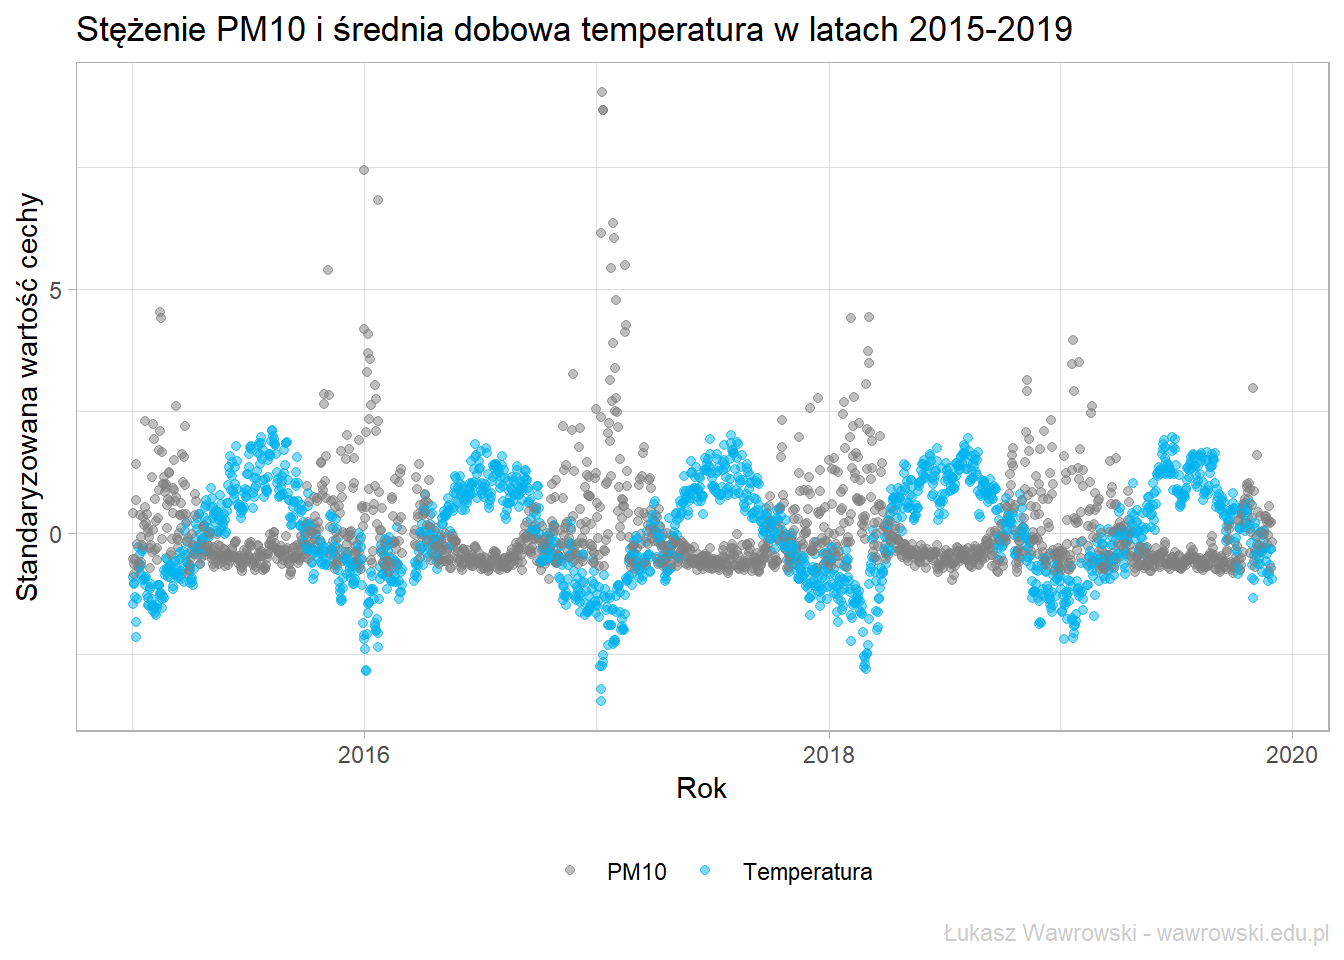
\includegraphics{Wawrowski_ADR_files/figure-latex/unnamed-chunk-14-1.pdf}

Wyżej wykorzystana funkcja jako kryterium odstawania przyjmuje wartość 3
identyfikując 4 obserwacje wpływowe. Z kolei dodanie do powyższej
funkcji przyrostka \emph{fit} powoduje przyjęcie jako granicy wartości
równej 2.

\begin{Shaded}
\begin{Highlighting}[]
\NormalTok{obs_wplyw <-}\StringTok{ }\KeywordTok{ols_plot_resid_stud_fit}\NormalTok{(wybrany_model)}
\end{Highlighting}
\end{Shaded}

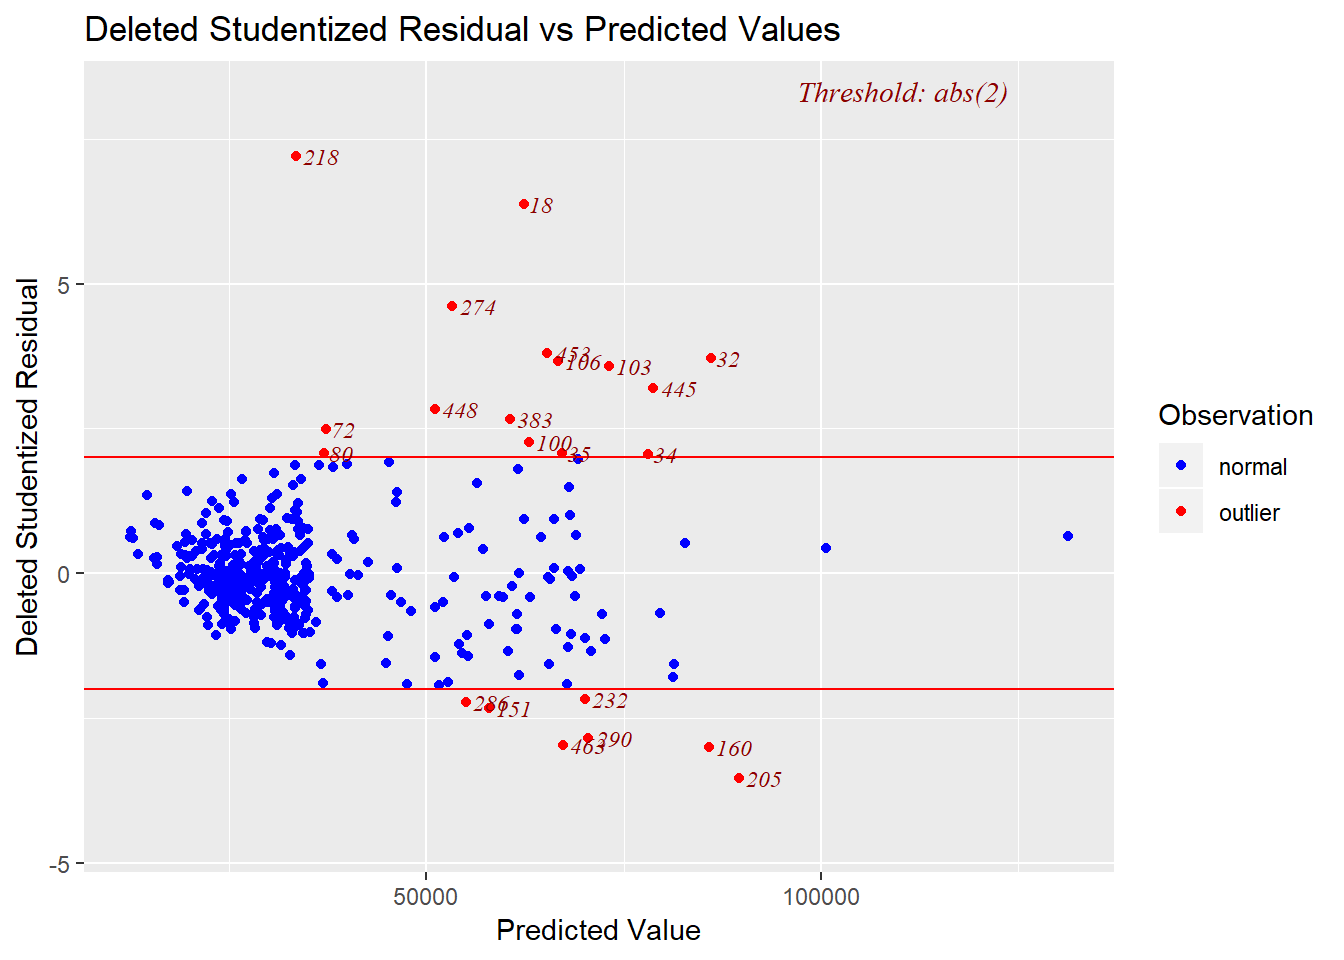
\includegraphics{Wawrowski_ADR_files/figure-latex/unnamed-chunk-15-1.pdf}

W ten sposób zostało zidentyfikowanych 10 obserwacji odstających.
Korzystając z tego ostatniego podejścia wyeliminujemy obserwacje
odstające ze zbioru uczącego:

\begin{Shaded}
\begin{Highlighting}[]
\NormalTok{nr_obs_wplyw <-}\StringTok{ }\NormalTok{obs_wplyw}\OperatorTok{$}\NormalTok{outliers}\OperatorTok{$}\NormalTok{observation}

\NormalTok{bez_obs_wplyw <-}\StringTok{ }\NormalTok{pracownicy2[}\OperatorTok{-}\NormalTok{nr_obs_wplyw,]}

\NormalTok{wybrany_model_out <-}\StringTok{ }\KeywordTok{lm}\NormalTok{(bwynagrodzenie }\OperatorTok{~}\StringTok{ }\NormalTok{pwynagrodzenie }\OperatorTok{+}\StringTok{ }\NormalTok{kat_pracownika }\OperatorTok{+}\StringTok{ }\NormalTok{doswiadczenie }\OperatorTok{+}\StringTok{ }\NormalTok{staz }\OperatorTok{+}\StringTok{ }\NormalTok{plec }\OperatorTok{+}\StringTok{ }\NormalTok{edukacja, }
                        \DataTypeTok{data =}\NormalTok{ bez_obs_wplyw)}
\KeywordTok{summary}\NormalTok{(wybrany_model_out)}
\end{Highlighting}
\end{Shaded}

\begin{verbatim}
## 
## Call:
## lm(formula = bwynagrodzenie ~ pwynagrodzenie + kat_pracownika + 
##     doswiadczenie + staz + plec + edukacja, data = bez_obs_wplyw)
## 
## Residuals:
##      Min       1Q   Median       3Q      Max 
## -12997.6  -2816.4   -481.4   2544.6  15180.2 
## 
## Coefficients:
##                    Estimate  Std. Error t value             Pr(>|t|)    
## (Intercept)     -4307.25866  2381.76657  -1.808             0.071217 .  
## pwynagrodzenie      1.39451     0.05382  25.908 < 0.0000000000000002 ***
## kat_pracownika2  6097.12115  1102.15833   5.532   0.0000000542431348 ***
## kat_pracownika3  9129.16469   972.97899   9.383 < 0.0000000000000002 ***
## doswiadczenie     -18.87447     2.41685  -7.810   0.0000000000000419 ***
## staz              120.56289    21.88184   5.510   0.0000000610683928 ***
## plec1           -1483.93151   521.34920  -2.846             0.004628 ** 
## edukacja          384.58159   109.81914   3.502             0.000509 ***
## ---
## Signif. codes:  0 '***' 0.001 '**' 0.01 '*' 0.05 '.' 0.1 ' ' 1
## 
## Residual standard error: 4592 on 443 degrees of freedom
## Multiple R-squared:  0.8986, Adjusted R-squared:  0.897 
## F-statistic:   561 on 7 and 443 DF,  p-value: < 0.00000000000000022
\end{verbatim}

Model dopasowny na takim zbiorze charakteryzuje się dużo mniejszym
błędem standardowym oraz wyższym współczynnikiem \(R^2\). Sprawdźmy w
takim razie normalność reszt.

\begin{Shaded}
\begin{Highlighting}[]
\KeywordTok{ols_plot_resid_qq}\NormalTok{(wybrany_model_out)}
\end{Highlighting}
\end{Shaded}

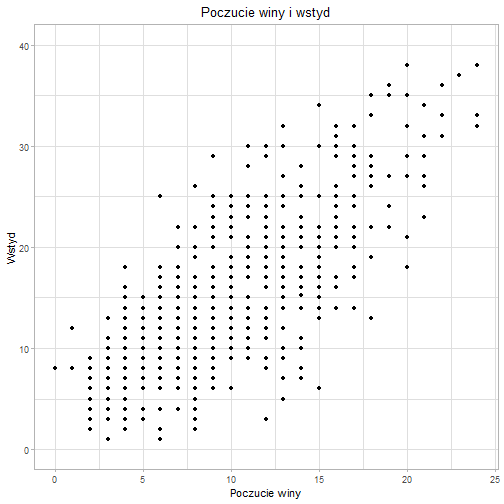
\includegraphics{Wawrowski_ADR_files/figure-latex/unnamed-chunk-17-1.pdf}

Wykres kwantyl-kwantyl wygląda już dużo lepiej, ale dla pewności
przeprowadzimy testy statystyczne.

\begin{Shaded}
\begin{Highlighting}[]
\KeywordTok{ols_test_normality}\NormalTok{(wybrany_model_out)}
\end{Highlighting}
\end{Shaded}

\begin{verbatim}
## -----------------------------------------------
##        Test             Statistic       pvalue  
## -----------------------------------------------
## Shapiro-Wilk              0.9708         0.0000 
## Kolmogorov-Smirnov        0.0675         0.0328 
## Cramer-von Mises         39.1404         0.0001 
## Anderson-Darling          3.8103         0.0000 
## -----------------------------------------------
\end{verbatim}

Tylko jeden test wskazał zgodność rozkładu reszt z rozkładem normalnym.

\subsection{Zadanie}\label{zadanie-1}

Na podstawie zbioru dotyczącego \href{data/50_Startups.csv}{50
startupów} określ jakie czynniki w największym stopniu wpływają na
przychód startupów.

\begin{Shaded}
\begin{Highlighting}[]
\NormalTok{startupy <-}\StringTok{ }\KeywordTok{read.csv}\NormalTok{(}\StringTok{"data/50_Startups.csv"}\NormalTok{)}

\KeywordTok{summary}\NormalTok{(startupy)}
\end{Highlighting}
\end{Shaded}

\begin{verbatim}
##    R.D.Spend      Administration   Marketing.Spend         State   
##  Min.   :     0   Min.   : 51283   Min.   :     0   California:17  
##  1st Qu.: 39936   1st Qu.:103731   1st Qu.:129300   Florida   :16  
##  Median : 73051   Median :122700   Median :212716   New York  :17  
##  Mean   : 73722   Mean   :121345   Mean   :211025                  
##  3rd Qu.:101603   3rd Qu.:144842   3rd Qu.:299469                  
##  Max.   :165349   Max.   :182646   Max.   :471784                  
##      Profit      
##  Min.   : 14681  
##  1st Qu.: 90139  
##  Median :107978  
##  Mean   :112013  
##  3rd Qu.:139766  
##  Max.   :192262
\end{verbatim}

\chapter{Grupowanie}\label{grupowanie}

Metody grupowania są wykorzystywane np. do segmentacji klientów, w
przypadku, gdy nie jest znany końcowy podział.

\section{Metoda k-średnich}\label{metoda-k-srednich}

Algorytm:

\begin{enumerate}
\def\labelenumi{\arabic{enumi}.}
\tightlist
\item
  Wskaź liczbę grup \(k\).
\item
  Wybierz dowolne \(k\) punktów jako centra grup.
\item
  Przypisz każdą z obserwacji do najbliższego centroidu.
\item
  Oblicz nowe centrum grupy.
\item
  Przypisz każdą z obserwacji do nowych centroidów. Jeśli któraś
  obserwacja zmieniła grupę - przejdź do kroku nr 4, a w przeciwnym
  przypadku zakończ algorytm.
\end{enumerate}

Zalety:

\begin{itemize}
\tightlist
\item
  dobrze działa zarówno na małych, jak i dużych zbiorach
\item
  efektywny
\end{itemize}

Wady:

\begin{itemize}
\tightlist
\item
  trzeba wskazać liczbę grup
\item
  losowy wybór punktów początkowych
\end{itemize}

\section{Metoda hierarchiczna}\label{metoda-hierarchiczna}

Algorytm:

\begin{enumerate}
\def\labelenumi{\arabic{enumi}.}
\tightlist
\item
  Każda obserwacji stanowi jedną z \(N\) pojedyńczych grup.
\item
  Na podstawie macierzy odległości połącz dwie najbliżej leżące
  obserwacje w jedną grupę (\(N-1\) grup).
\item
  Połącz dwa najbliżej siebie leżące grupy w jedną (\(N-2\) grup).
\item
  Powtórz krok nr 3, aż do uzyskania jednej grupy.
\end{enumerate}

Zalety:

\begin{itemize}
\tightlist
\item
  prosty sposób ustalenia liczby grup
\item
  praktyczny sposób wizualizacji
\end{itemize}

Wady:

\begin{itemize}
\tightlist
\item
  nieodpowiedni dla dużych zbiorów
\end{itemize}

\subsection{Zadanie}\label{zadanie-2}

Na podstawie zbioru zawierającego informacje o
\href{data/klienci.csv}{klientach sklepu} dokonaj grupowania klientów.

Opis zbioru:

\begin{itemize}
\tightlist
\item
  klientID - identyfikator klienta
\item
  plec - płeć
\item
  wiek - wiek
\item
  roczny\_dochod - roczny dochód wyrażony w tys. dolarów
\item
  wskaznik\_wydatkow - klasyfikacja sklepu od 1 do 100
\end{itemize}

\href{res/grupowanie.Rmd}{grupowanie.Rmd}

\href{res/adr.zip}{cały projekt}

\subsection{Zadanie 2}\label{zadanie-2-1}

Dokonaj grupowania danych dotyczących \href{data/auta.csv}{32
samochodów} według następujących zmiennych: pojemność, przebieg, lata
oraz cena.

\subsection{Zadanie 3}\label{zadanie-3}

Rozpoznawanie czynności na podstawie danych z przyspieszeniomierza w
telefonie:
\href{http://archive.ics.uci.edu/ml/datasets/User+Identification+From+Walking+Activity\#}{User
Identification From Walking Activity Data Set}

\chapter{Klasyfikacja}\label{klasyfikacja}

\href{http://www.r2d3.us/visual-intro-to-machine-learning-part-1/}{A
visual introduction to machine learning} - niestety powstała tylko jedna
część.

\section{Drzewa klasyfikacyjne}\label{drzewa-klasyfikacyjne}

Zalety:

\begin{itemize}
\tightlist
\item
  łatwa interpretacja
\item
  nie trzeba normalizować cech
\item
  rozwiązuje problemy liniowe i nieliniowe
\end{itemize}

Wady:

\begin{itemize}
\tightlist
\item
  mała efektywność przy małych zbiorach danych
\item
  łatwo można przeuczyć
\end{itemize}

\section{KNN}\label{knn}

Algorytm:

\begin{enumerate}
\def\labelenumi{\arabic{enumi}.}
\tightlist
\item
  Określ liczbę sąsiadów - \(K\)
\item
  Wyznacz \(K\) sąsiadów dla nowego punktu na podstawie wybranej
  odległości
\item
  Oblicz liczbę sąsiadów, w każdej z grup
\item
  Przypisz nową obserwację do grupy, w której ma więcej najbliższych
  sąsiadów
\end{enumerate}

Zalety:

\begin{itemize}
\tightlist
\item
  łatwa interpretacja
\item
  szybki i efektywny
\end{itemize}

Wady:

\begin{itemize}
\tightlist
\item
  trzeba określić liczbę sąsiadów
\end{itemize}

\subsection{Zadanie}\label{zadanie-4}

Zbuduj model klasyfikacyjny dla zbioru
\href{data/Social_Network_Ads.csv}{danych} dotyczących cech internautów
oraz informacji czy zamówili reklamowany produkt czy nie.

Przeprowadź imputację braków danych dla zbioru
\href{data/pracownicy.RData}{pracowników}.

\chapter{Materiały z zajęć}\label{materiay-z-zajec}

\section{28.10.2018}\label{section}

\href{res/skrypt20181028.R}{Wprowadzenie do R}

\href{res/analiza20181028.R}{Analiza sejmików}

\section{18.11.2018}\label{section-1}

\href{https://departmentofstatisticspue.github.io/statystyka-opisowa/analiza-struktury.html}{Analiza
struktury}

\href{data/rossmann.xlsx}{Rossmann}

\href{res/zajecia20181118.R}{Analiza struktury w R}

\section{16.12.2018}\label{section-2}

\href{prezentacje/03.html}{Prezentacja}

\href{data/Salary_Data.csv}{Pracownicy}

\href{res/korelacje20181216.R}{Korelacja w R}

\href{res/regresja20181216.Rmd}{Regresja w R}

\section{26.01.2019}\label{section-3}

\href{data/salary.xlsx}{Pensja i doświaczenie}

\href{data/pracownicy.xlsx}{Pracownicy}

Opis zbioru:

\begin{itemize}
\tightlist
\item
  id - kod pracownika
\item
  plec - płeć pracownika (0 - mężczyzna, 1 - kobieta)
\item
  data\_urodz - data urodzenia
\item
  edukacja - wykształcenie (w latach nauki)
\item
  kat\_pracownika - grupa pracownicza (1 - ochroniarz, 2 - urzędnik, 3 -
  menedżer)
\item
  bwynagrodzenie - bieżące wynagrodzenie
\item
  pwynagrodzenie - początkowe wynagrodzenie
\item
  staz - staż pracy (w miesiącach)
\item
  doswiadczenie - poprzednie zatrudnienie (w miesiącach)
\item
  zwiazki - przynależność do związków zawodowych (0 - nie, 1 - tak)
\item
  wiek - wiek (w latach)
\end{itemize}

\href{res/regresja20190126.R}{Regresja w R}


\end{document}
